\section{Results and Discussion}

To verify the chaotic nature of the double pendulum, we used the RK4 method as follows:
We initialized two \textit{almost} identical double pendulum systems (sharing identical lengths $l_1,l_2$ and masses $m_1,m_2$) with initial angles differing by a microscopic perturbation, $\epsilon$.
\[\Theta_A=(\theta_1,\theta_2)\quad\text{and}\quad \Theta_B=(\theta_1+\epsilon,\theta_2)\]
where $\epsilon = 10^{-5}$ degrees.

\figref{10-5} illustrates the trajectories of these two systems over time. During the first few sections, the deviation caused by the perturbation appears negligible, and the two systems move in unison. However, as the system moves forward, the non-linear coupling terms in the equations of motion, specifically those derived in \eqref{eq:rearr1}, cause this infinitesimal difference $\epsilon$ to propagate and grow exponentially for some time.

\begin{figure}[h]
  \centering
    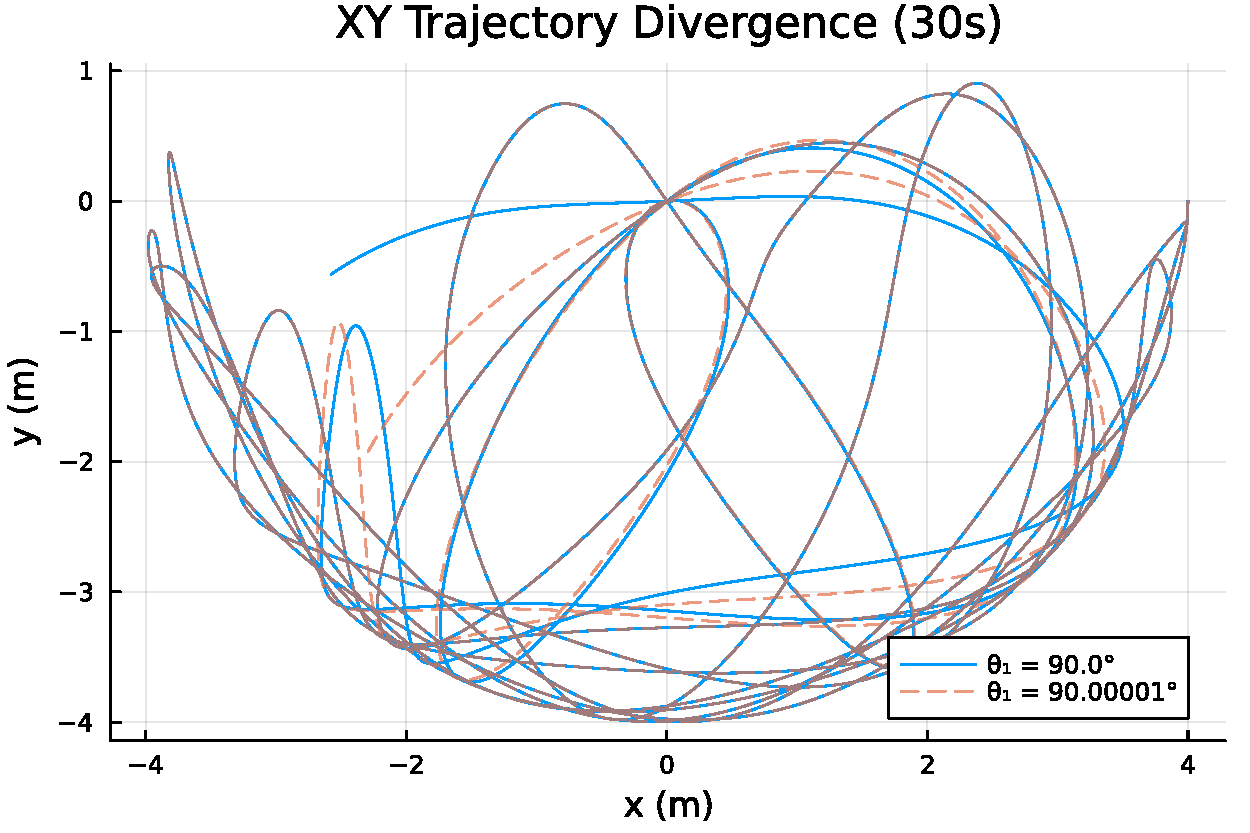
\includegraphics[width=0.8\textwidth]{Figures/xy_divergence.pdf}
    \caption{Divergence of trajectories with initial conditions differing by $10^{-5}$ degrees.}
    \figlabel{10-5}
\end{figure}

By the end of the simulation, the two pendulums exhibit completely uncorrelated behavior. This confirms that while the double pendulum is deterministic (fully described by Equations \ref{ddtheta1} and \ref{ddtheta2}), it is practically unpredictable over long time horizons due to this extreme sensitivity.

Plotting the angular difference $\Delta\theta$ between the two systems further illustrates this chaotic dissociation. As shown in \figref{dt}, the error does not grow linearly but exhibits rapid, unpredictable fluctuations, the peaks of which grow exponentially, a characteristic of the butterfly effect.
\begin{figure}[H]
  \centering
    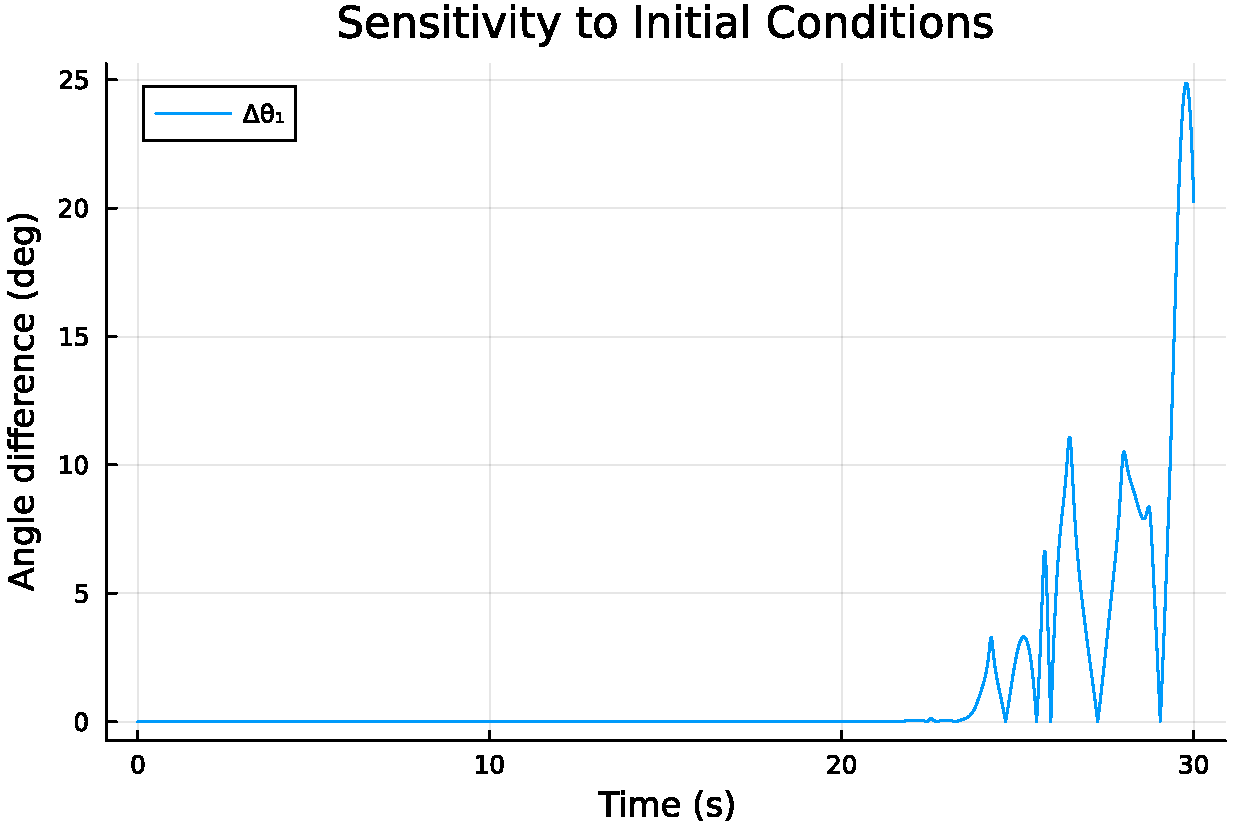
\includegraphics[width=0.8\textwidth]{Figures/dt.pdf} 
    \caption{Evolution of the angular difference $\Delta\theta$ between the two systems over time.}
    \figlabel{dt}
\end{figure}

The results validate that simple physical systems can exhibit complex, non-intuitive behavior. Future work could involve solving triple or \(n\)-pivot pendulums. This would require much higher-dimension vector fields to incorporate into the methods. Further study on \(n\)-pivot pendulums would also require analysis of whether RK4 is accurate enough for such systems.
